\documentclass[a4paper,11pt]{article}
\usepackage[spanish]{babel}
\usepackage[utf8]{inputenc}

% Configuración páginas
\usepackage{vmargin}							% Márgenes

\usepackage{sectsty}							% Fuente de los títulos
\allsectionsfont{\normalfont \Large \scshape}

\usepackage{graphicx}							% Imágenes
\graphicspath{{images/}}

\usepackage{tabularx}							% Otras
\usepackage{multirow}							% Celdas ocupando varias filas

\usepackage{mathtools}							% Matematicas
\newcommand\numberthis{							% numeración en align*
	\addtocounter{equation}{1}\tag{\theequation}
}

\usepackage{algorithm,algpseudocode}			% Algoritmos en latex
\makeatletter
\renewcommand{\ALG@name}{Algoritmo}				% Cambiamos la palabra "Algorithm"
\makeatother
\algnewcommand\Input{\item[\textbf{Entrada:}]}
\let\oldReturn\Return
\renewcommand{\Return}{\State\oldReturn}

% Configuración del título
\newcommand{\horrule}[1]{\rule{\linewidth}{#1}} 	% Horizontal rule

\title{
	\vspace{-25pt}
	\normalfont \Large \textsc{
		Modelos de Investigación Operativa,
        Ingeniería Informática\\
        Universidad de Valladolid
	}\\[10pt]
	\horrule{1pt}\\[10pt]
	\huge \textbf{
		Práctica 12
	}\\
	\horrule{1pt}
}
\author{
	\normalfont \Large Daniel González Alonso
}
\date{
	\normalfont \large \today
}

%%%%%%%%%%%%%%%%%%%%%%%%%%%%%%%%%%%%%%%%%%%%%%%%%%
\begin{document}
\maketitle

%%%% RESUMEN %%%%
\begin{abstract}
	En este documento se describen los problemas y los resultados obtenidos de la práctica 12 del tema 5 de la asignatura Modelos de Investigación Operativa de Ingeniería Informática, Universidad de Valladolid.
\end{abstract}

%%%% DESARROLLO %%%%
\section{Introducción}
Esta práctica trata de problemas TSP (\textit{Travelling Salesman Problem}). Los problemas TSP constan de un grafo ${G=(N,A)}$, donde ${N}$ son los nodos del grafo y ${A}$ los arcos entre éstos, con un coste asociado por cada arco, y el objetivo consiste en encontrar el camino Hamiltoniano (un camino que pase por todos los nodos) de coste mínimo.\\

En esta práctica se nos pide implementar la solución al problema TSP mediante la metaheurística \textit{GRASP}. El pseudocódigo de la esta metaheurística se muestra a continuación:

\begin{algorithm}[!htbp]
\caption{Metaheurística \textit{GRASP}}
\label{alg_grasp}
\begin{algorithmic}[1]
\Function{GRASP}{${N}$}
    \State ${f^{\ast} \gets \infty}$
    \For{${i \gets 1,N}$}
        \State ${x \gets \Call{SoluciónGreedy}{\null}}$
        \State ${x \gets \Call{BúsquedaLocal}{x}}$
        \If{${f(x) < f^{\ast}}$}
            \State ${f^{\ast} \gets f(x)}$
            \State ${x^{\ast} \gets x}$
        \EndIf
    \EndFor
	\Return{${x^{\ast}}$}
\EndFunction
\end{algorithmic}
\end{algorithm}

En nuestro caso, ${N}$ es el número máximo de iteraciones, ${\Call{SoluciónGreedy}{\null}}$ es la solución de la heurística del entorno y ${\Call{BúsquedaLocal}{x}}$ es el algoritmo \textit{2-opt}.

%%%%%%%%%%%%%%%%%%%%%%%%%%%%%%%%%%%%%%%%%%%%%%%%%%%%%%
\newpage
\section{Desarrollo}
En esta práctica hay que programar la heurística \textit{GRASP} partiendo de la solución que proporciona la heurística del entorno más cercano (comenzando en un nodo aleatoriamente escogido) y aplicarlo a los 5 ejemplos de ${n=21}$ nodos y los 6 problemas Euclídeos de las prácticas anteriores. Parámetros sugeridos: ${N}$ = 30, 60 y 100, y ${K = 5}$.\\

Estos problemas se encuentran resueltos mediante \textit{Xpress Mosel} en los ficheros \texttt{tsp \ \_grasp\_n21\_1.mos}, \texttt{tsp\_grasp\_n21\_2.mos}, \texttt{tsp\_grasp\_n21\_3.mos}, \texttt{tsp\_grasp\_n21\_4.mos}, \texttt{tsp\_grasp\_n21\_5.mos} en el caso de los ficheros \texttt{n21} y por otro lado para los ficheros \texttt{tsp} Euclídeos en los ficheros \texttt{tsp\_grasp\_tsp\_60\_1.mos}, \texttt{tsp\_grasp\_tsp\_60\_2.mos}, \texttt{tsp\_grasp\_ \ tsp\_60\_3.mos}, \texttt{tsp\_grasp\_tsp\_100\_1.mos}, \texttt{tsp\_grasp\_tsp\_100\_2.mos} y \texttt{tsp\_grasp\_tsp\_ \ 100\_3.mos} (el nombre indica el fichero de datos empleado).\\

Antes de explicar la implementación del algoritmo cabe destacar que los costes ${c_{i,j}}$ en nuestro caso son distancias. Para los ficheros \texttt{n21} la matriz de distancias nos viene dada en el mismo fichero. En el caso de los ficheros \texttt{tsp} solo nos vienen las coordenadas de cada nodo, por ello antes de empezar con estos últimos ficheros hay que calcular la matriz de distancias. Para estos fichero la matriz se calculo mediante la distancia Euclídea redondeada al entero más cercano. En caso de la distancia de un nodo a si mismo, se introducía en esta matriz en vez de 0 un valor ``infinito'' (\texttt{MAX\_INT}).\\

Una vez obtenidos los costes, lo primero que se hizo fue un bucle que itera entre los valores de ${N}$ que nos pide el enunciado (30, 60, y 100). Dentro de ese bucle se ejecuta la solución \textit{GRASP} con cada valor de ${N}$.\\

Para implementar la solución \textit{GRASP} siguiendo el esquema \ref{alg_grasp}, primero definí una variable llamada \texttt{distancia\_minima} (${f^{\ast}}$ en el esquema superior) así como un vector \texttt{siguientes} los cuales almacenan la mejor solución encontrada por el algoritmo. Después cree un bucle que se ejecuta ${N}$ veces, el cual en cada iteración hace lo siguiente:

\begin{enumerate}
\item Obtener una solución Greedy: Para esta parte reutilicé el código de la práctica 10 donde se obtenía una solución Greedy mediante la heurística del entorno más cercano.
\item Hacer la búsqueda local: Para hacer la búsqueda local en el entorno de la solución obtenida por el algoritmo Greedy utilizamos la mejora \textit{2-opt}. Para esta parte utlicé el mismo código que el empleado para la práctica 11.
\item Actualizar la solución óptima: En esta parte, en caso de que la distancia total obtenida en los pasos anteriores sea mejor que \texttt{distancia\_minima} actualizamos este valor así como el vector \texttt{siguientes} con la solución de la iteración actual.
\end{enumerate}

%%%%%%%%%%%%%%%%%%%%%%%%%%%%%%%%%%%%%%%%%%%%%%%%%%%%%%
\newpage
\section{Resultados}
Los resultados obtenidos para los ficheros de datos de esta práctica fueron los siguientes:

\begin{table}[!htbp]
\label{results_n21}
\centering
\begin{tabularx}{\textwidth}{|p{2cm}|X|X|X|X|X|}
\hline
\multirow{2}{*}{Valor de N}  &   \multicolumn{5}{|c|}{Problema TSP}  \\ \cline{2-6}
	& \texttt{n21\_1}	& \texttt{n21\_2}	& \texttt{n21\_3}	& \texttt{n21\_4}	& \texttt{n21\_5} \\ \hline
30	& 198   & 174   & 213   & 189   & 193   \\ \hline
60	& 198   & 174   & 213   & 189   & 193   \\ \hline
100	& 198   & 174   & 213   & 189   & 193   \\ \hline
\end{tabularx}
\caption{Comparación de las distancias totales obtenidas con distintos valores de ${N}$ para los ficheros \texttt{n21}}
\end{table}

\begin{table}[!htbp]
\label{results_tsp}
\centering
\begin{tabularx}{\textwidth}{|p{2cm}|X|X|X|X|X|X|}
\hline
\multirow{2}{*}{Valor de N}  &   \multicolumn{6}{|c|}{Problema TSP}  \\ \cline{2-7}
	& \texttt{tsp\_60\_1}	& \texttt{tsp\_60\_2}	& \texttt{tsp\_60\_3}	& \texttt{tsp\_100\_1}	& \texttt{tsp\_100\_2}	& \texttt{tsp\_100\_3} \\ \hline
30	&    633	& 611   & 592   & 779   & 787    & 815  \\ \hline
60	&    628	& 607   & 589   & 751   & 762    & 810  \\ \hline
100	&    632	& 614   & 586   & 760   & 777    & 789  \\ \hline
\end{tabularx}
\caption{Comparación de las distancias totales obtenidas con distintos valores de ${N}$ para los ficheros \texttt{tsp}}
\end{table}

También obtuve los gráficos IVE para los ficheros \texttt{tsp}. En este caso aquí se muestra una comparación de los resultados obtenidos para \texttt{tsp\_100\_1} con distintos valores de $N$:

\begin{table}[!htbp]
\label{images_100}
\centering
\begin{tabular}{|p{2cm}|c|}
\hline
Valor de $N$	& Solución \textit{GRASP}	\\ \hline
30 & 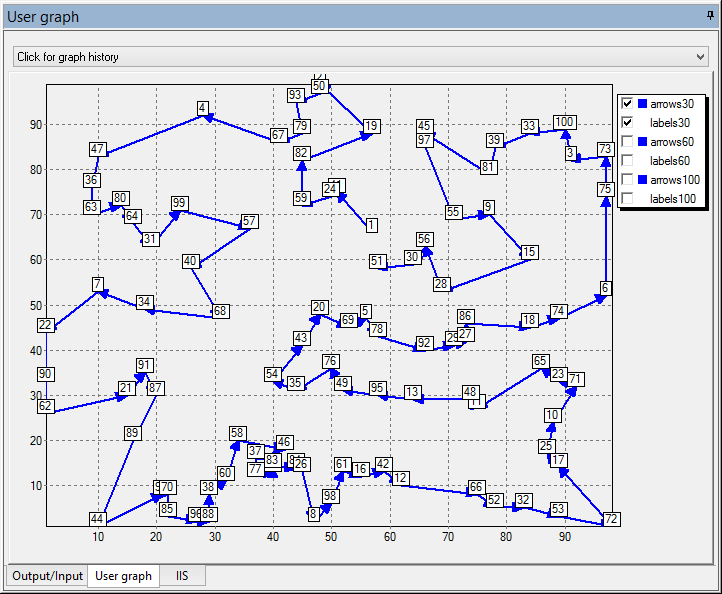
\includegraphics[width=6.5cm]{images//grasp_100_1_n30.png}	\\ \hline
60 & 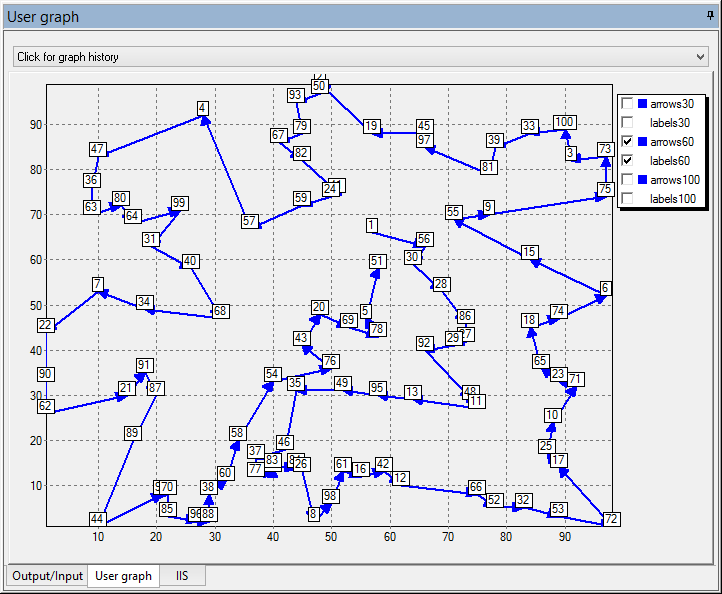
\includegraphics[width=6.5cm]{images/grasp_100_1_n60.png}	\\ \hline
100 & 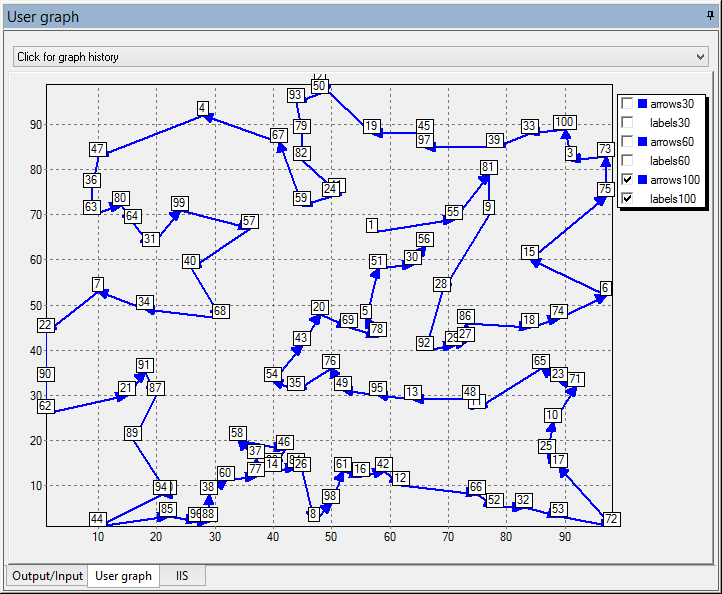
\includegraphics[width=6.5cm]{images/grasp_100_1_n100.png}	\\ \hline
\end{tabular}
\caption{Comparación de los caminos obtenidos con distintos valores de ${N}$ para el ficheros \texttt{tsp\_100\_1.txt}}
\end{table}

\end{document}
